
\documentclass[aps,twocolumn,secnumarabic,nobalancelastpage,amsmath,amssymb,
nofootinbib]{revtex4}

% nofootinbib is another document class option that allows you to put
% footnotes on the page where they occur rather than at the end of the
% paper.  This makes for easier reading!

% secnumarabic is a particularly nice way of identifying sections by
% number to aid electronic review and commentary.

% amsmath and amssymb are necessary for the subequations environment
% among others

\usepackage{chapterbib}
\usepackage{color}
\usepackage{graphics}      % standard graphics specifications
\usepackage{graphicx}      % alternative graphics specifications
\usepackage{longtable}     % helps with long table options
%\usepackage{url}          % for on-line citations (conflicts with hyperref)
\usepackage{bm}            % special 'bold-math' package
\usepackage[colorlinks=true]{hyperref}


\begin{document}
\title{The Frank-Hertz Experiment}
\author         {Adnan Basar (Partner: Kadir Simsek)}
\email          {adnanbasarr@icloud.com}
\affiliation    {2010205108}
\date{\today}





\begin{abstract}
In this experiment, we are going to measure an important phenomena encountered in collisions between electrons and atoms: quantized excitation due to inelastic scattering.
\end{abstract}

\maketitle

%%%%%%%%%%%%%%%%%%%%%%%%%%%%%%%%%%%%%%%%%%%%%%%%%%%%%%%%%%%%%%%%%%
\section{Introduction}

Franck and Hertz described the first observation of quantized excitation in 1914, one year after Bohr published his theory of the hydrogen atom with its concept of
quantized energy states. They discovered that electrons
moving through mercury vapor with an energy greater
than or equal to a critical value near 4.9 eV can excite
the 2536 $\AA$ line of the mercury spectrum. Electrons with
less than the critical energy bounce elastically when they
collide with mercury atoms and fail to excite any electromagnetic emission. The experiment provided crucial
evidence in favor of the Bohr theory. This graph easily shows that excitation levels.

\begin{figure}[htbp]
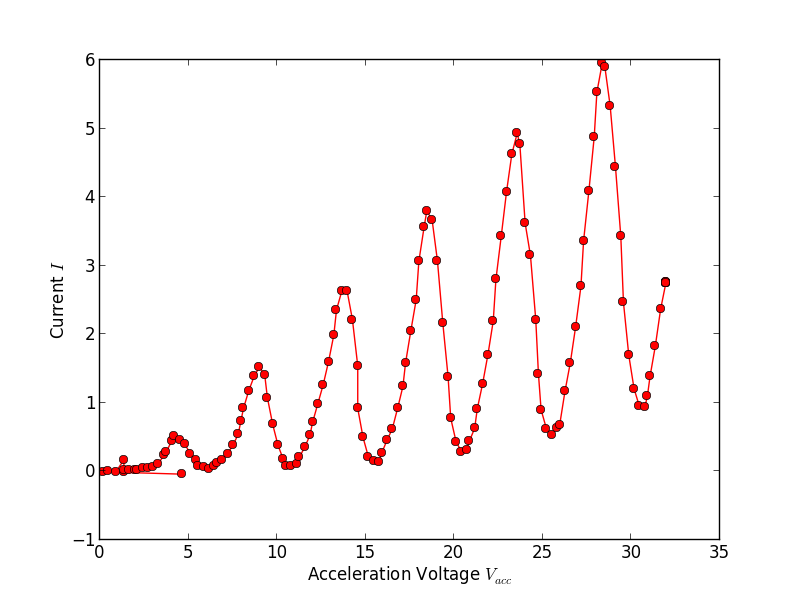
\includegraphics[width=3in]{sample}
\caption{Excitation levels of electrons through mercury vapor}
\label{fig:schematic}
\end{figure}

\subsection{Contact Potential}

Consideration of contact potentials is also necessary. In simple terms, this means that the 
accelerating potential is not completely converted into kinetic energy of the electrons: some of it 
provides the “work function” of the cathode material, i.e. the amount of energy (measured in 
electron volts) necessary to free the electrons from the cathode. The cathode is coated with a 
material with a relatively low work function. The collector plate, since it is used merely as 
electron collector, has a somewhat higher work function. The contact potential is the difference 
between the work functions, since they are oppositely directed in the electric field, that is, the 
electric field has to work against the cathode potential but is helped in the case of the collector 
plate. Thus we should expect that the voltage to the first peak will be greater than the average 
peak to peak voltage, due to the contact potential. The contact potential can be calculated as the 
average peak to peak voltage subtracted from the first peak voltage. 


\section{Experimental Setup}

\begin{figure}[htbp]
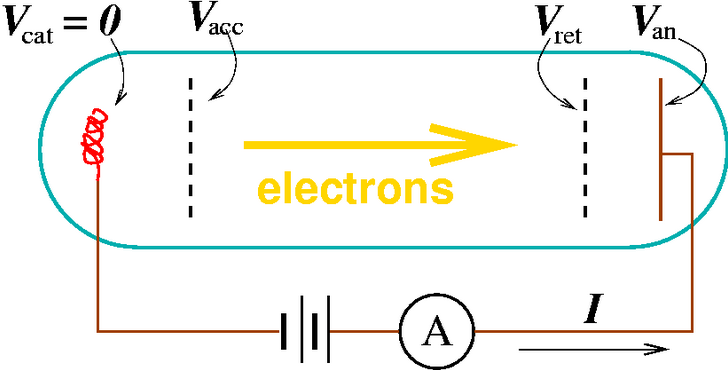
\includegraphics[width=3in]{experiment}
\caption{Franck-Hertz Tube}
\label{fig:schematic}
\end{figure}

In this experiment we used such items as:

\begin{itemize}
\item Franck-Hertz Tube
\item DC Power Supply
\item Current Amplifier
\item AC filament Power Supply
\item Temperature Probe with Display
\item Electric Oven with The Special Copper Tube and The Power Supply
\end{itemize}

\begin{figure}[htbp]
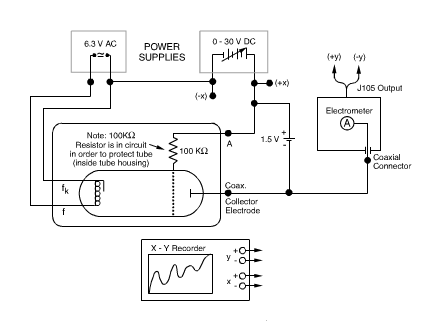
\includegraphics[width=3in]{experiment2}
\caption{Schematized Setup}
\label{fig:schematic}
\end{figure}




\section{Data and Analysis}


We have data from five 5 different temperatures as in the tables:





\begin{center}
\begin{table}[htbp]
\begin{tabular}{|l|c|c|r|}
\hline
{\small Temperature ($C$)} & {\small $V_1$(1.5 $V$)} & {\small $V_2$(2.0 $V$)} & {\small $V_3$(2.5 $V$)} \\
\hline
		& 7.05 V 		& 6.45 V& 	6.15 V \\
 		& 12.15 V		& 11.70 V & 11.25 V \\
155 	& 17.25 V 		& 16.95 V & 16.65 V \\
 		& 22.80 V 		& 22.35 V & 21.90 V \\
 		& 28.20 V 		& 27.75 V & 27.15 V \\

\hline
\end{tabular}
\caption{\label{tab:linfitresults} For Temperature 155 C }
\end{table}
\end{center}

\begin{center}
\begin{table}[htbp]
\begin{tabular}{|l|c|c|r|}
\hline
{\small Temperature ($C$)} & {\small $V_1$(1.5 $V$)} & {\small $V_2$(2.0 $V$)} & {\small $V_3$(2.5 $V$)} \\
\hline
		& 7.05 V 		& 6.45 V& 	6.00 V \\
 		& 11.85 V		& 11.40 V & 10.95 V \\
165 	& 16.95 V 		& 16.65 V & 15.90 V \\
 		& 22.05 V 		& 21.75 V & 21.00 V \\
 		& 27.45 V 		& 26.85 V & 26.40 V \\

\hline
\end{tabular}
\caption{\label{tab:linfitresults} For Temperature 165 C}
\end{table}
\end{center}

\begin{center}
\begin{table}[htbp]
\begin{tabular}{|l|c|c|r|}
\hline
{\small Temperature ($C$)} & {\small $V_1$(1.5 $V$)} & {\small $V_2$(2.0 $V$)} & {\small $V_3$(2.5 $V$)} \\
\hline
		& 7.05 V 		& 6.60 V& 	6.00 V \\
 		& 11.85 V		& 11.25 V & 11.10 V \\
175 	& 16.95 V 		& 16.50 V & 16.05 V \\
		& 22.20 V 		& 21.60 V & 21.15 V \\
 		& 27.45 V 		& 27.15 V & 26.40 V \\

\hline
\end{tabular}
\caption{\label{tab:linfitresults} For Temperature  175 C}
\end{table}
\end{center}

\begin{center}
\begin{table}[htbp]
\begin{tabular}{|l|c|c|r|}
\hline
{\small Temperature ($C$)} & {\small $V_1$(1.5 $V$)} & {\small $V_2$(2.0 $V$)} & {\small $V_3$(2.5 $V$)} \\
\hline
		& 6.75 V 		& 6.45 V& 	6.00 V \\
 		& 11.55 V		& 11.25 V & 10.95 V \\
185 	& 16.65 V 		& 16.05 V & 15.90 V \\
 		& 21.45 V 		& 21.15 V & 20.85 V \\
 		& 26.70 V 		& 26.25 V & 25.80 V \\

\hline
\end{tabular}
\caption{\label{tab:linfitresults} For Temperature 185 C }
\end{table}
\end{center}

\begin{center}
\begin{table}[htbp]
\begin{tabular}{|l|c|c|r|}
\hline
{\small Temperature ($C$)} & {\small $V_1$(1.5 $V$)} & {\small $V_2$(2.0 $V$)} & {\small $V_3$(2.5 $V$)} \\
\hline
		& 7.05 V 		& 6.60 V& 	6.30 V \\
 		& 11.70 V		& 11.40 V & 11.10 V \\
195 	& 16.65 V 		& 16.20 V & 15.60 V \\
 		& 21.45 V 		& 21.15 V & 20.85 V \\
 		& 26.40 V 		& 25.95 V & 25.65 V \\

\hline
\end{tabular}
\caption{\label{tab:linfitresults} For Temperature  195 C}
\end{table}
\end{center}

For each division of tables, we are going to calculate

\begin{itemize}



\item $\Delta{V}={V}_{i+1}-{V}_{i}$

\item Avarage: $(\Delta{V})_{mean}=\frac{1}{N}{\sum{\Delta{V}_i}}$
\item Standard Deviation-Squared: ${\sigma_{\Delta{V}}}^{2}=\frac{1}{N-1}{\sum{{\Delta{V_i}-\Delta{V}_{mean}}^{2}}}$

\end{itemize}

For all values, we have following results in table.


\begin{center}
\begin{table}[htbp]
\begin{tabular}{|l|c|c|r|}
\hline
{\small Voltage ($V$)} & {\small Temp. ($C$)} & {\small $\Delta{V}_{mean}$ ($V$)} & {\small $\sigma_{\Delta{V}}^{2}$ ($V^{2}$)} \\
\hline
1.5		&  	155	& 5.28 & 	0.050 \\
2.0		&  	155	& 5.32 & 	0.007 \\
2.5		&  	155	& 5.25 & 	0.014 \\
1.5		&  	165	&  5.1 & 	0.059 \\
2.0		&  	165	&  5.1 & 	0.014 \\
2.5		&  	165	&  5.1 & 	0.044  \\
1.5		&  	175	&  5.1& 	 0.044\\
2.0		&  	175	&  5.13& 	 0.140\\
2.5		&  	175	&  5.1& 	 0.014\\
1.5		&  	185	&  4.98& 	 0.050\\
2.0		&  	185	&  4.95& 	 0.029\\
2.5		&  	185	&  4.85& 	 0.044\\
1.5		&  	195	&  4.83& 	 \~\ 0\\
2.0		&  	195	&  4.83& 	 0.005\\
2.5		&  	195	&  4.83& 	 0.095\\


\hline
\end{tabular}
\caption{\label{tab:linfitresults} Results of Mean and Standard Deviation Squared Calculations}
\end{table}
\end{center}

\begin{center}
${V}_{weighted}=\frac{\sum{\frac{\Delta{V_i}}{\sigma_{\Delta{V_i}}^2}}}{\sum{\frac{1}{\sigma{\Delta{V_{i}}}^2}}}=5.05\ V$
\end{center}

\begin{center}
${\sigma}_{weighted}^2=\frac{1}{\sum{\frac{1}{\sigma{\Delta{V_{i}}}^2}}}=0.001\ V^2$
\end{center}

$\sigma_{instrumental}$ is given as 0.05 $V$.

$\sigma_{total}^2=\sigma_{weighted}^2+\sigma_{instrumental}^2= 0.0038\ V^2 $

$\sigma_{total}=0.061\ V$

\section{Results}
In results part, the true value for the voltage difference is 4.9 eV. We have found as: 5.05 V and $\sigma_{total}=0.061\ V$

\begin{center}
Error:$\frac{abs(4.9-5.05)}{0.61}=2.56\ \sigma$ range.
\end{center}

\section{Conclusion}

We obtained a value that is very close to true value, but actually with error calculation, it is not a good idea to make estimations by using our experiment. We could not take precise data from experiment since fluctuations of temperature does not allow. $\sigma$ shows that this result in easy observation.


\section{References}
\begin{itemize}
\item E. Gulmez, ”Advanced Physics Experiment”, Istanbul, Bogazici University Publication, 1999
\item http://web.mit.edu/8.13/www/experiments.shtml
\end{itemize}



\bibliography{photoelectric}


%%%%%%%%%%%%%%%%%%%%%%%%%%%%%%%%%%%%%%%%%%%%%%%%%%%%%%%%%%%%%%%%%%%%%%%%%%%%%
\begin{acknowledgments}

I would like to thank my partner Kadir Simsek for his help to the experiment, and also to the teaching assistant Merve Tarman for her guidance during the experiment.
\end{acknowledgments}

%%%%%%%%%%%%%%%%%%%%%%%%%%%%%%%%%%%%%%%%%%%%%%%%%%%%%%%%%%%%%%%%%%%%%%%%%%%%%

\end{document}
